%
\section{The Fundamental Data Structures within LocalRegions}

As mentioned earlier, in almost all object-oriented languages (which includes $C++$), there exists the concepts of {\em class attributes} and {\em object attributes}.   For a summary of attributes and access patterns, please review Section \ref{sec:stdregions-datastructures}.
Within the LocalRegions directory of the library, there exists a class inheritance hierarchy designed to try to encourage re-use of core
algorithms (while simultaneously trying to minimize duplication of code).  We present this class hierarchy in Figure \ref{localregions:localclasstree}.


\begin{figure}[htb]
\centering
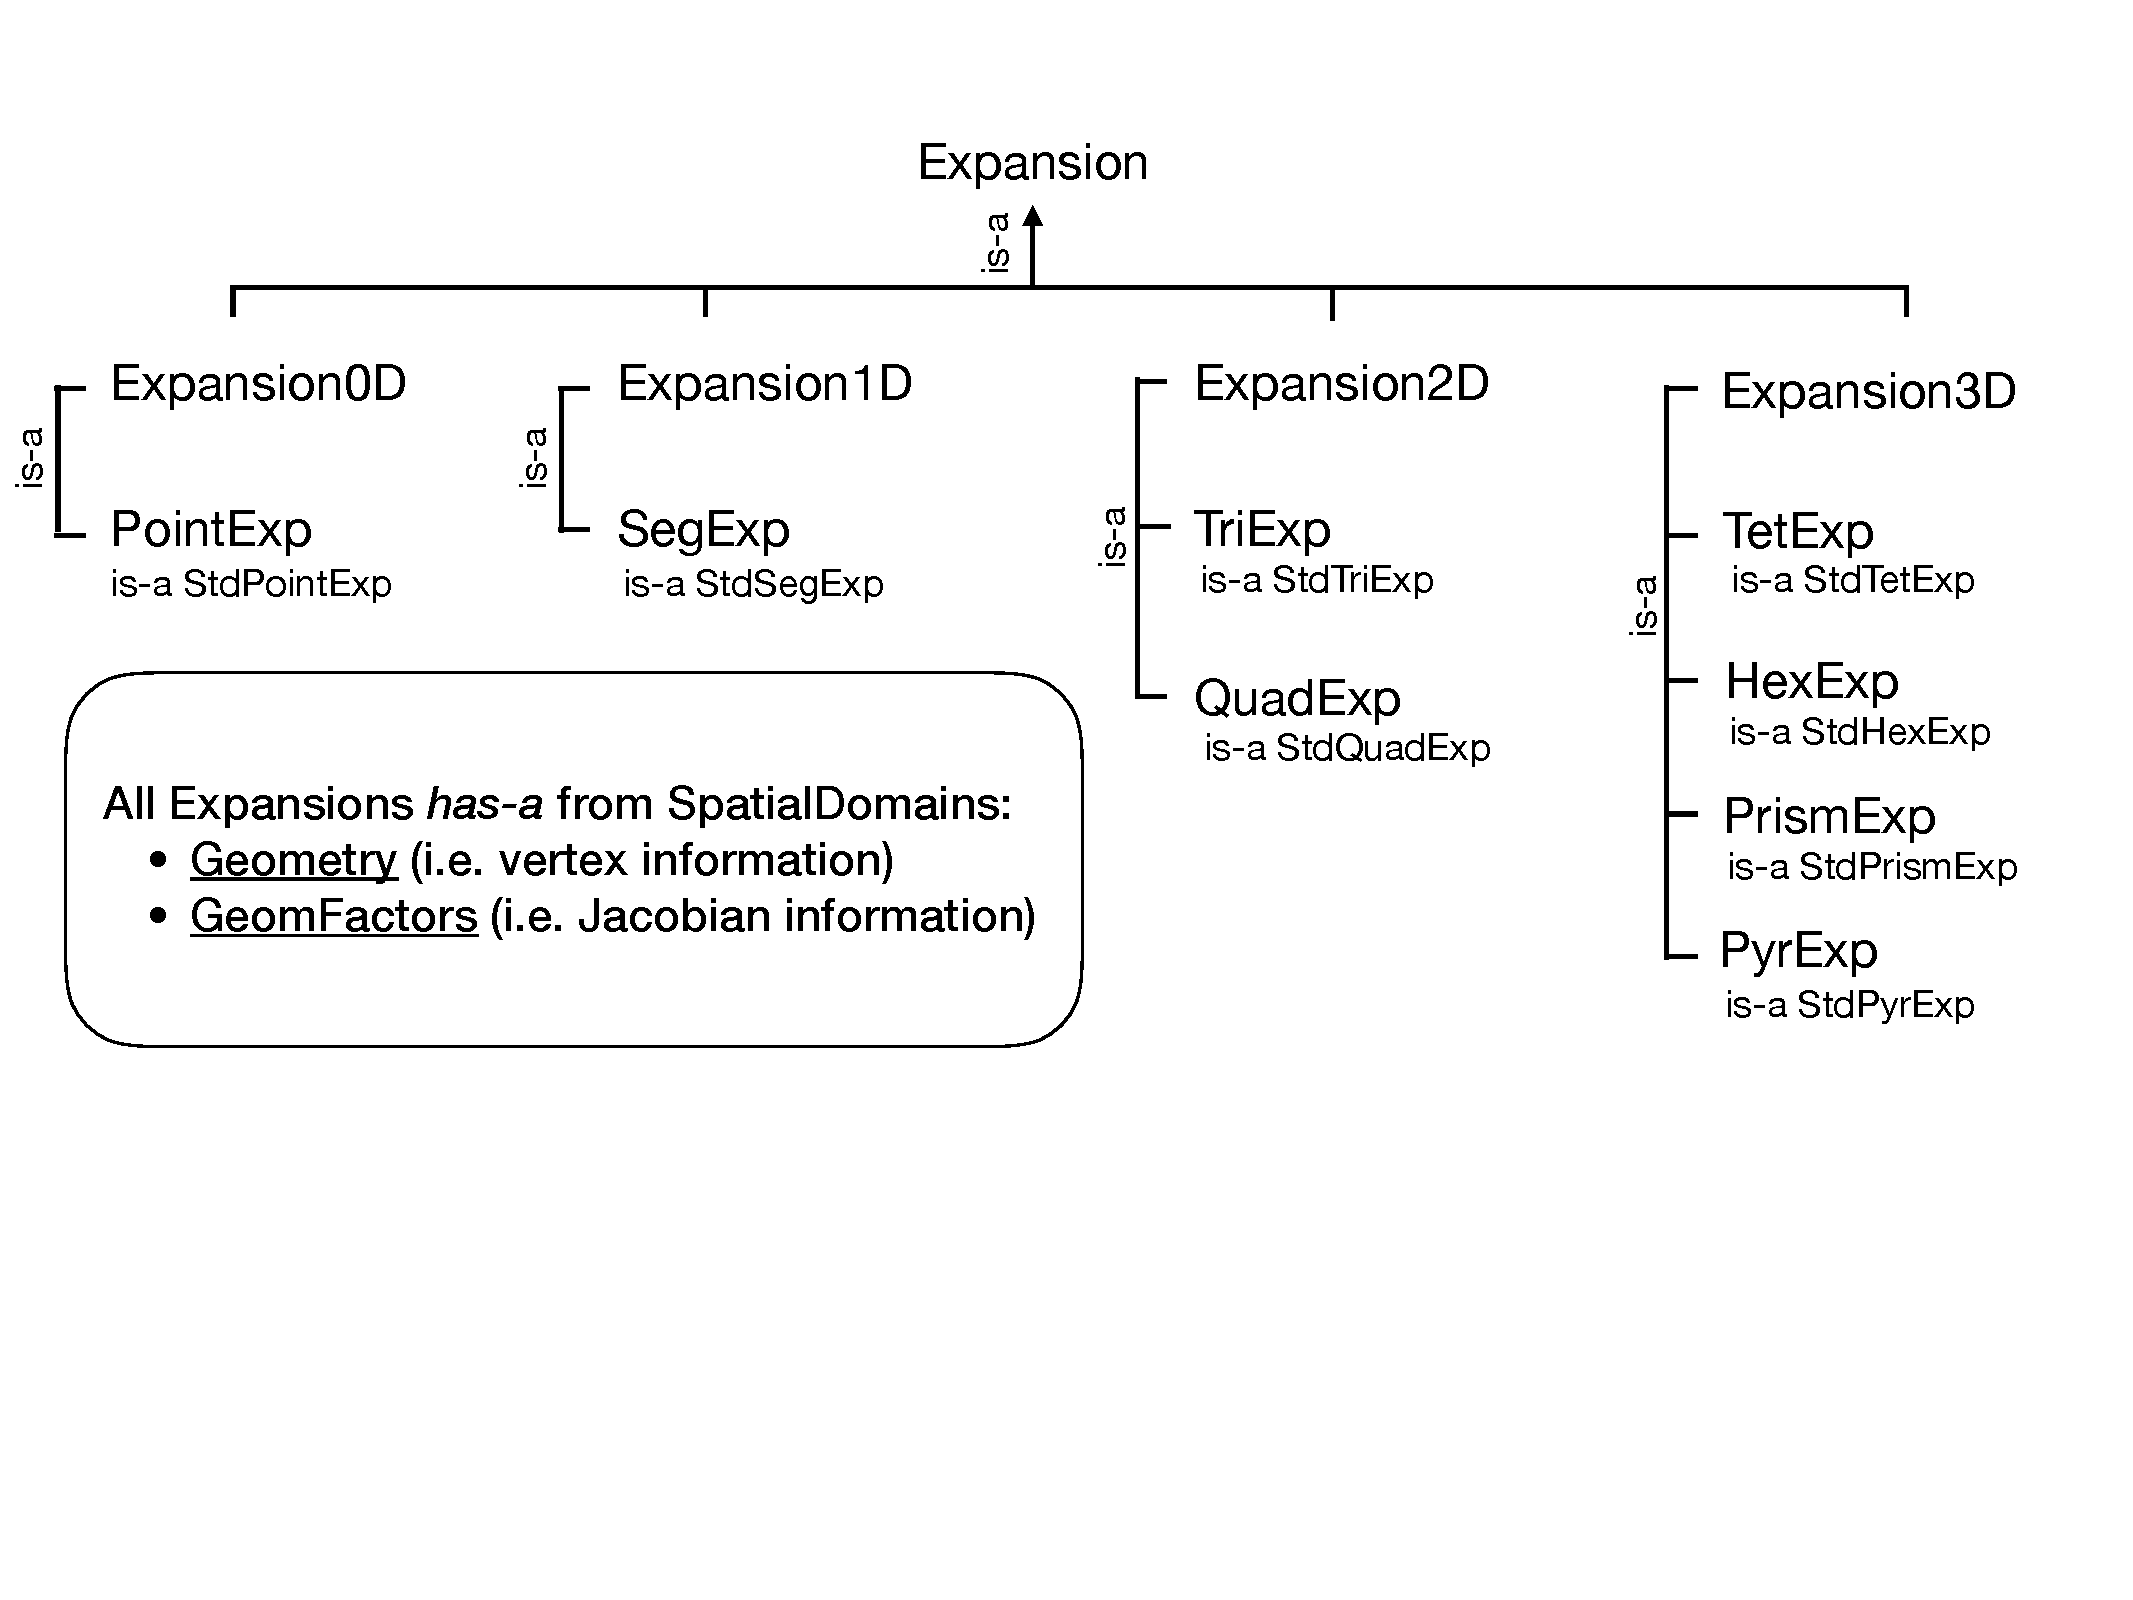
\includegraphics[width=6in]{img/expansiontree.pdf}
\caption{Class hierarchy derived from Expansion, the base class of the LocalRegions Directory.}
\label{localregions:localclasstree}
\end{figure}

As is seen in Figure \ref{stdregions:localclasstree}, the LocalRegions hierarchy consists of three levels:  the base level from which all
LocalRegion objects are derived is Expansion.   This object is then specialized by dimension, yielding Expansion0D, 
Expansion1D, Expansion2D and Expansion3D.  The dimension-specific objects are then specialized based upon
shape.  

The object attributes (variables) at various levels of the hierarchy can be understood in light of Figure \ref{stdregions:stdexpansion}.
At its core, an expansion is a means of representing a function over a world-space region evaluated at a collection of point positions.
The various data members hold information to allow all these basic building blocks to be specified.  Many of the attributes are 
inherited from StdRegions as they are not unique to LocalRegions; however, each LocalRegion Expansion is uniquely defined based
upon its geometric factors (which it stores via SpatialDomain information).


\begin{figure}[htb]
\centering
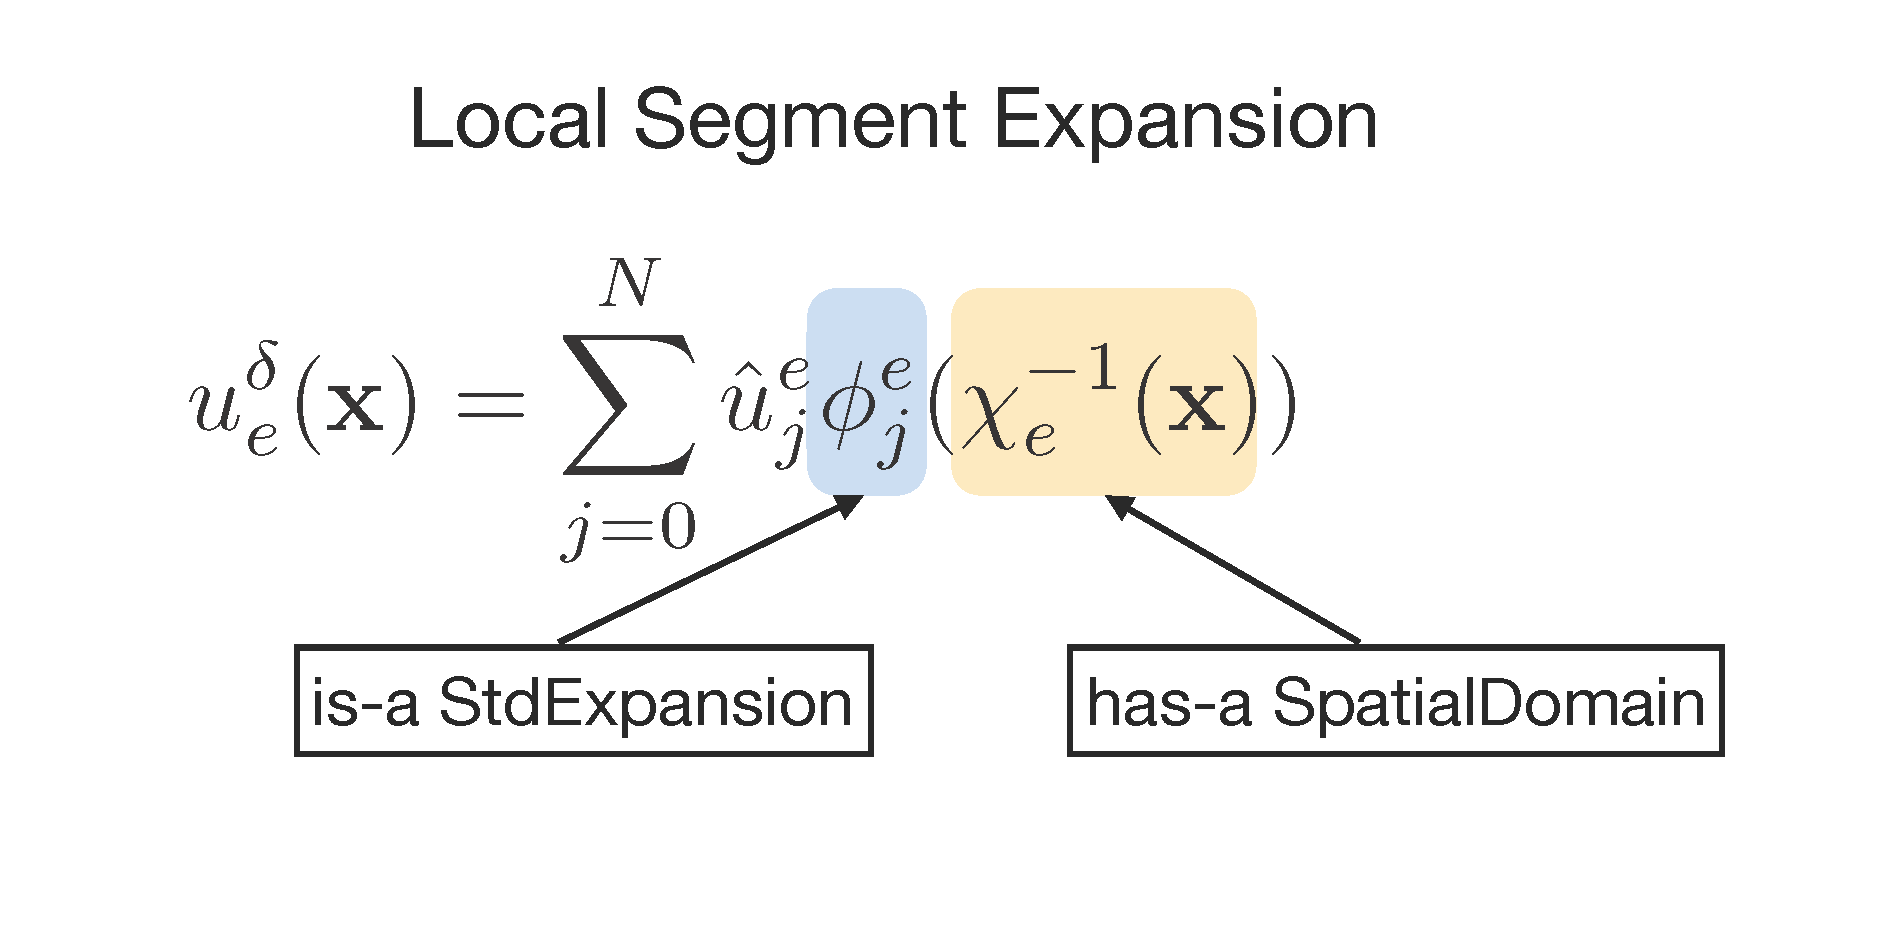
\includegraphics[width=6in]{img/LocalExpansion.png}
\caption{Diagram to help understand the various data members (object attributes) contained within LocalRegions and how they connect with the mathematical representation presented earlier.  Recall that a LocalRegion {\em is-a} StdRegion and {\em has-a} SpatialDomain.}
\label{localregions:localexpansion:stdexpansion}
\end{figure}

The various private, protected and public data members contained within LocalRegions are provided in the subsequent sections.

%%%%%%%%%%%%%%%%%%%%%%%%%%%%%%%%%%%%%%%%
\subsection{Variables at the Level of Expansion}

\paragraph{Private:}

There are private methods but no private data members within Expansion.

\paragraph{Protected:}

As discussed above, the primary data in LocalRegions that distinguishes it from StdExpansions is the {\em has-a} relationship with SpatialDomains, given by the following:

\begin{itemize}
\item SpatialDomains::GeometrySharedPtr  \verb+m_geom+
%
\item SpatialDomains::GeomFactorsSharedPtr \verb+m_metricinfo+
%
\item MetricMap \verb+m_metrics+
\end{itemize}


\paragraph{Public:}

There are public methods but no public data members within Expansion.


%%%%%%%%%%%%%%%%%%%%%%%%%%%%%%%%%%%%%%%%
\subsection{Variables at the Level of Expansion\$D for various Dimensions}
\paragraph{Private:}

\paragraph{Protected:}

\paragraph{Public:}


%%%%%%%%%%%%%%%%%%%%%%%%%%%%%%%%%%%%%%%%
\subsection{Variables at the Level of Shape-Specific Expansions}

\paragraph{Private:}

\paragraph{Protected:}

\paragraph{Public:}

